\section{Cônicas}

\subsection*{Completamento de Quadrados}


\begin{frame}[label=comp]
	\frametitle{Completamento de Quadrados}
	%\begin{scriptsize}
	
\begin{block}{Produto Notáveis}
	\[(x+k)^2=x^2+2k\cdot x+k^2\]
	\[(x-k)^2=x^2-2k\cdot x+k^2\]
\end{block}	

\begin{exe}
	Resolva as seguintes equações sem usar a fórmula de Bhaskara
	\begin{multicols}{2}
		\begin{enumerate}
			\item $x^2-x=0$
			\item $4x^2-1=0$
			\item $x^2-2x=8$
			\item $x^2-8x=9$
		\end{enumerate}
	\end{multicols}
	\medskip
\end{exe}

\end{frame}


\begin{frame}[label=comp]
	\begin{exe}
Complete os quadrados:
\begin{enumerate}
	\item $x^2+7x$
	\item $-2x^2+8x$
\end{enumerate}
	\end{exe}

\begin{block}{Fórmula de Bhaskara}
	Sejam  $a,b$ e $c\in\R$ com $a\neq 0$. Então as soluções da equação $ax^2+bx+c=0$ são dadas por
	\[ x=\frac{-b\pm \sqrt{b^2-4ac}}{2a}\]
\end{block}
\end{frame}

\begin{frame}[label=comp]
	
\begin{casa}
	Complete os quadrados:
\begin{enumerate}
	\item $x^2-4x$
	\item $-x^2+2x$
	\item $3x^2-9x$
\end{enumerate}
\end{casa}

\end{frame}


\subsection*{Cônicas}
\begin{frame}[label=conicas]{Cônicas}

 Uma \dt{cônica}, é uma curva obtida cortando-se um
cone circular reto por um plano. As cônicas mais importantes são
as \dt{elipses, as hipérboles e as parábolas}, que ocorrem quando o plano 
cortante não passa pelo vértice do cone.

\begin{center}
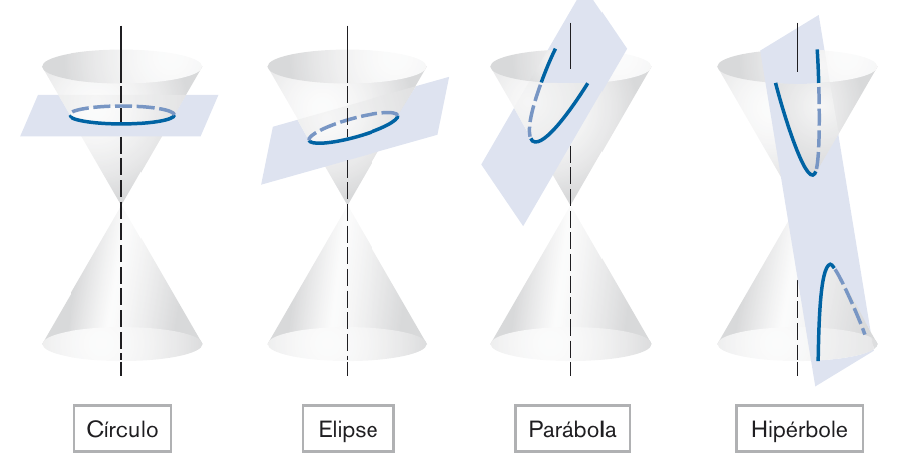
\includegraphics[scale=.4]{figuras/conicas.png}
\end{center}
%
%Os círculos são casos especiais de elipses, que resultam quando o
%plano cortante é perpendicular ao eixo de simetria do cone. Se o plano 
%cortante passa pelo vértice, então a interseção resultante é denominada uma 
%cônica degenerada, cujas possibilidades são um ponto, um par de retas que 
%se cortam ou uma única reta.
\end{frame}


\begin{frame}[label=conicas]

Em um plano cartesiano, uma equação da forma
\begin{equation*}
{\color{blue}a}{x^2}+{\color{blue}b}{y^2}
+{\color{blue}c}{xy}+{\color{blue}d}{x}
+{\color{blue}e}{y}+{\color{blue}f}=0
\end{equation*}
com \dt{$a,b$} e \dt{$c$} não todos nulos, representam uma cônica, onde também 
estão incluídos os casos das chamadas \dt{cônicas degeneradas}, cujas 
possibilidade são: \dt{um ponto}, \dt{um par de retas}, \dt{uma única 
reta} ou \dt{o conjunto vazio}.

\begin{exe}
São exemplos de cônicas que já conhecemos:
\begin{enumerate}
\item $x^2+2x-y=0$ é uma parábola.
\item $x^2+y^2=1$ é um círculo.
\item $x^2+y^2+1=0$ é o conjunto vazio.
\end{enumerate}
Qual cônica é essa
\[x^2+y^2+4x+3=0?\]
\end{exe}

\end{frame}

\subsection*{Cônicas na forma Reduzida}
\begin{frame}[label=conicas]{Cônicas na forma reduzida}
Para cada cônica, podemos escolher um sistema de eixos cartesianos de modo que a equação que a represente assuma a forma mais simples possível, chamada de \dt{equação reduzida (ou canônica)}.

\begin{itemize}
\item Elipse: $\dps\frac{x^2}{a^2}+\frac{y^2}{b^2}=1$;

\item Hipérbole: $\dps\frac{x^2}{a^2}-\frac{y^2}{b^2}=1$ ou $\dps\frac{y^2}{b^2}-\frac{x^2}{a^2}=1$;

\item Parábola: $y=ax^2$ ou $x=ay^2$.
\end{itemize}
\end{frame}


\subsection*{Elipse}
\begin{frame}[label=conicas]{Elipse}
\begin{center}
\textcolor{red}{\fbox{$\displaystyle\frac{x^2}{a^2}+\frac{y^2}{b^2}=1$}}
\end{center}
\begin{minipage}{0.4\textwidth}
	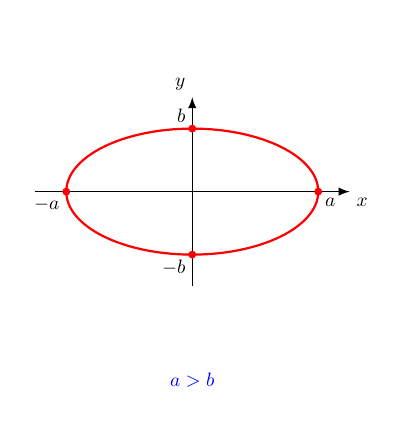
\begin{tikzpicture}[scale=0.8, every node/.style={scale=0.7}]
\node at (0,2.5) { };
	\draw[->] (-2.5,0) -- (2.5,0);
	\draw[->] (0,-1.5) -- (0,1.5);
	\node[below right] at (2.5,0) {$x$};
	\node[above left] at (0,1.5) {$y$};		
	\draw[thick,red] (0,0) ellipse (2cm and 1cm);
	\draw[fill,red] (2,0) circle (1.5pt);   	
	\draw[fill,red] (-2,0) circle (1.5pt);
	\draw[fill,red] (0,1) circle (1.5pt);   	
	\draw[fill,red] (0,-1) circle (1.5pt);
	\node[below right] at (2,0) {$a$};
	\node[below left] at (-2,0) {$-a$};
	\node[left] at (0,1.2) {$b$};
	\node[left] at (0,-1.2) {$-b$};
	\node[blue] at (0,-3) {$\displaystyle a>b$};
	\end{tikzpicture}
\end{minipage}
\begin{minipage}{0.25\textwidth}
	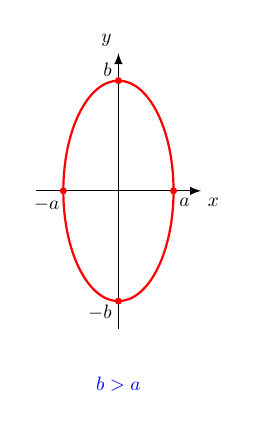
\begin{tikzpicture}[scale=0.7, every node/.style={scale=0.7}]
	\draw[->] (0,-2.5) -- (0,2.5);
	\draw[->] (-1.5,0) -- (1.5,0);
	\node[below right] at (1.5,0) {$x$};
	\node[above left] at (0,2.5) {$y$};		
	\draw[thick,red] (0,0) ellipse (1cm and 2cm);
%	\draw[fill,blue] (0,1.3) circle (1.5pt);
%	\draw[fill,blue] (0,-1.3) circle (1.5pt);   
%	\node[left] at (0,1.3) {$c$};
%	\node[left] at (0,-1.3) {$-c$};
	\draw[fill,red] (0,2) circle (1.5pt);   	
	\draw[fill,red] (0,-2) circle (1.5pt);
	\draw[fill,red] (1,0) circle (1.5pt);   	
	\draw[fill,red] (-1,0) circle (1.5pt);
	\node[left] at (0,2.2) {$b$};
	\node[left] at (0,-2.2) {$-b$};
	\node[below] at (1.2,0) {$a$};
	\node[below] at (-1.3,0) {$-a$};
	\node[blue] at (0,-3.5) {$\displaystyle b>a$};
	\end{tikzpicture}
\end{minipage}
\begin{minipage}{0.2\textwidth}
	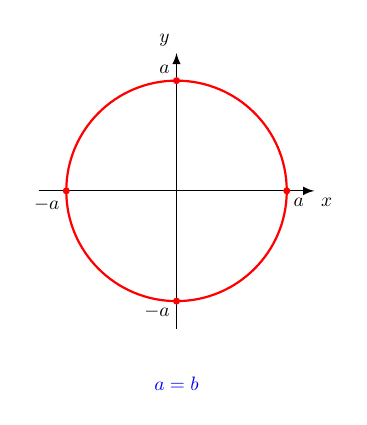
\begin{tikzpicture}[scale=0.7, every node/.style={scale=0.7}]
	\draw[->] (-2.5,0) -- (2.5,0);
	\draw[->] (0,-2.5) -- (0,2.5);
	\node[below right] at (2.5,0) {$x$};
	\node[above left] at (0,2.5) {$y$};		
	\draw[thick,red] (0,0) ellipse (2cm and 2cm);
	\draw[fill,red] (2,0) circle (1.5pt);   	
	\draw[fill,red] (-2,0) circle (1.5pt);
	\draw[fill,red] (0,2) circle (1.5pt);   	
	\draw[fill,red] (0,-2) circle (1.5pt);
	\node[below right] at (2,0) {$a$};
	\node[below left] at (-2,0) {$-a$};
	\node[left] at (0,2.2) {$a$};
	\node[left] at (0,-2.2) {$-a$};
	\node[blue] at (0,-3.5) {$\displaystyle a=b$};
	\end{tikzpicture}
\end{minipage}

\end{frame}

\subsection*{Hipérbole}
\begin{frame}[label=conicas]{Hipérbole}
%\begin{center}
%\textcolor{red}{\fbox{$\displaystyle\frac{x^2}{a^2}-\frac{y^2}{b^2}=1$}}
%\end{center}
 \ \ \ \ \ \begin{minipage}{0.6\textwidth}
\qquad\quad
{\color{red}\fbox{$\displaystyle\frac{x^2}{a^2}-\frac{y^2}{b^2}=1$}}
\bigskip

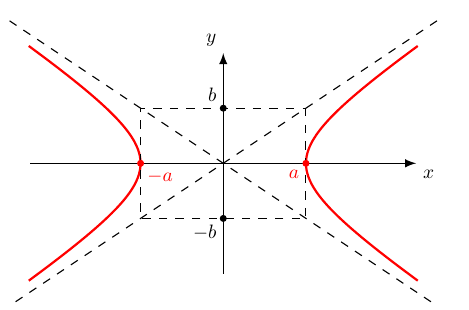
\begin{tikzpicture}[scale=0.7, every node/.style={scale=0.7}]
\def\a{1.5}	
\def\b{1}			

\coordinate (AB) at (\a,\b);
\coordinate (ABm) at (-\a,-\b);
\coordinate (mAB) at (-\a,\b);
\coordinate (AmB) at (\a,-\b);

%\node[red] at (0,4) {$\displaystyle\frac{x^2}{a^2}-\frac{y^2}{b^2}=1$};
\draw[domain=-1.5:1.5,smooth,variable=\t,red,thick]
plot ({\a*cosh(\t )},{\b*sinh(\t)});
\draw[domain=-1.5:1.5,smooth,variable=\t,red,thick]
plot ({-\a*cosh(\t )},{\b*sinh(\t)});

\draw[->] (-3.5,0) -- (3.5,0);
\draw[->] (0,-2.) -- (0,2);
\node[below right] at (3.5,0) {$x$};
\node[above left] at (0,2) {$y$};

\draw [shorten >= -2.cm, shorten <=-2.cm,dashed] (AB)--(ABm);
\draw [shorten >= -2.cm, shorten <=-2.cm,dashed] (mAB)--(AmB);
\draw[dashed] (AB) -- (AmB) -- (ABm) -- (mAB) -- (AB);

\draw[fill,red] (\a,0) node[below left] {$a$} circle (1.5pt);
\draw[fill,red] (-\a,0) node[below right] {$-a$} circle (1.5pt);

	\draw[fill] (0,\b) node[above left] {$b$} circle (1.5pt);
\draw[fill] (0,-\b) node[below left] {$-b$} circle (1.5pt);
\end{tikzpicture}
\end{minipage}
\begin{minipage}{0.3\textwidth}

{\color{red}\fbox{$\displaystyle\frac{y^2}{b^2}-\frac{x^2}{a^2}=1$}}
\bigskip

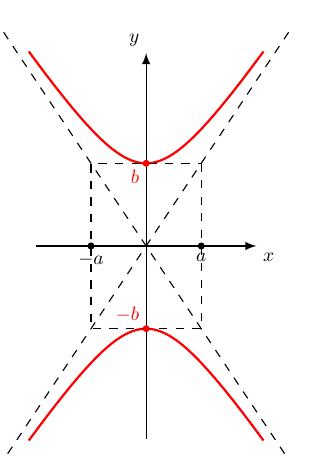
\begin{tikzpicture}[scale=0.7, every node/.style={scale=0.7}]	
\def\a{1.5}	
\def\b{1}		

\coordinate (AB) at (\b,\a);
\coordinate (ABm) at (-\b,-\a);
\coordinate (mAB) at (-\b,\a);
\coordinate (AmB) at (\b,-\a);		

\draw[domain=-1.5:1.5,smooth,variable=\t,red,thick]
plot ({\b*sinh(\t)},{\a*cosh(\t )});
\draw[domain=-1.5:1.5,smooth,variable=\t,red,thick]
plot ({\b*sinh(\t)},{-\a*cosh(\t )});

\draw[->] (0,-3.5) -- (0,3.5);
\draw[->] (-2,0) -- (2,0);
\node[below right] at (2,0) {$x$};
\node[above left] at (0,3.5) {$y$};

\draw [shorten >= -2.cm, shorten <=-2.cm,dashed] (AB)--(ABm);
\draw [shorten >= -2.cm, shorten <=-2.cm,dashed] (mAB)--(AmB);
\draw[dashed] (AB) -- (AmB) -- (ABm) -- (mAB) -- (AB);

\draw[fill,red] (0,\a) node[below left] {$b$} circle (1.5pt);
\draw[fill,red] (0,-\a) node[above left] {$-b$} circle (1.5pt);

\draw[fill] (\b,0) node[below] {$a$} circle (1.5pt);
\draw[fill] (-\b,0) node[below] {$-a$} circle (1.5pt);

\end{tikzpicture}
\end{minipage}
\end{frame}


\subsection*{Parábola}
\begin{frame}[label=conicas]{Parábola}

\qquad\begin{minipage}{0.5\textwidth}
\quad
{\footnotesize {\color{red}\fbox{$\displaystyle y=ax^2, \ a>0$}}}


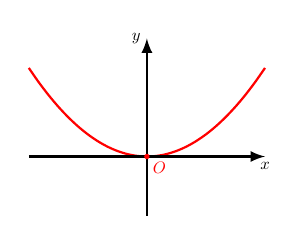
\begin{tikzpicture}[scale=0.5, every node/.style={scale=0.6}]	
	\def\p{1}	
\onslide<1->{\draw[scale=1,domain=-3:3,smooth,variable=\t,red,thick]
	plot ({\t},{\t*\t/(4*\p)});}
\draw[thick,->] (-3,0) -- (3,0) node[below] {$x$};
\draw[thick,->] (0,-1.5) -- (0,3) node[left] {$y$}; 
\draw[fill,red] (0,0) circle (1.5pt);
\node[below right,red] at (0,0) {$O$};

\end{tikzpicture}
\end{minipage}
\begin{minipage}{0.3\textwidth}
\quad
{\footnotesize {\color{red}\fbox{$\displaystyle y=-ax^2, \ a>0$}}}
\bigskip

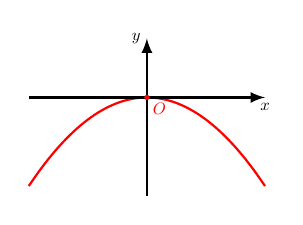
\begin{tikzpicture}[scale=0.5, every node/.style={scale=0.6}]
\def\p{1}	
\draw[scale=1,domain=-3:3,smooth,variable=\t,red,thick]
	plot ({\t},{-\t*\t/(4*\p)});

\draw[thick,->] (-3,0) -- (3,0) node[below] {$x$};
\draw[thick,->] (0,-2.5) -- (0,1.5) node[left] {$y$}; 
\draw[fill,red] (0,0) circle (1.5pt);
\node[below right,red] at (0,0) {$O$};

\end{tikzpicture}
\end{minipage}
\bigskip
\bigskip

\qquad\begin{minipage}{0.5\textwidth}
\quad
{\footnotesize {\color{red}\fbox{$\displaystyle x=ay^2, \ a>0$}}}


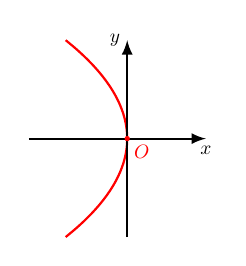
\begin{tikzpicture}[scale=0.5, every node/.style={scale=0.7}]
\def\p{1}	
\draw[scale=1,domain=-2.5:2.5,smooth,variable=\t,red,thick]
	plot ({-\t*\t/(4*\p)},{\t});
\draw[thick,->] (-2.5,0) -- (2,0) node[below] {$x$};
\draw[thick,->] (0,-2.5) -- (0,2.5) node[left] {$y$}; 
\draw[fill,red] (0,0) circle (1.5pt);
\node[below right,red] at (0,0) {$O$};

\end{tikzpicture}
\end{minipage}
\begin{minipage}{0.3\textwidth}
\qquad\quad
{\footnotesize {\color{red}\fbox{$\displaystyle x=-ay^2, \ a>0$}}}


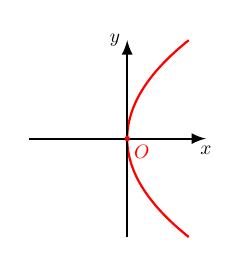
\begin{tikzpicture}[scale=0.5, every node/.style={scale=0.7}]	
\def\p{1}	
\draw[scale=1,domain=-2.5:2.5,smooth,variable=\t,red,thick]
	plot ({\t*\t/(4*\p)},{\t});
\draw[thick,->] (-2.5,0) -- (2,0) node[below] {$x$};
\draw[thick,->] (0,-2.5) -- (0,2.5) node[left] {$y$}; 
\draw[fill,red] (0,0) circle (1.5pt);
\node[below right,red] at (0,0) {$O$};

\end{tikzpicture}
\end{minipage}

\end{frame}

\begin{frame}[label=conicas]
\begin{exe}
Identifique as cônicas abaixo e faça um esboço.
\begin{enumerate}
\item $4x^2+9y^2=36$
\item $5x^2-2y^2=15$
\item $4x^2-9y=0$
\item $y^2=5x$
\end{enumerate}
\end{exe}

\end{frame}

\subsection*{Curvas que não são parábolas}
\begin{frame}[label=conicas]{Curvas que não são parábolas}
	\begin{enumerate}
		\item $y=x^4$
		\item $y=\cosh x=\frac{e^x+e^{-x}}{2}$  ( catenária ) 
	\end{enumerate}
	
	
	Quando um cabo flexível pesado é suspenso entre dois pontos  na mesma altura, vemos a formação de uma curva conhecida como \dest{catenária}, do latim \textit{catena} que significa corrente. 
	\begin{figure}
		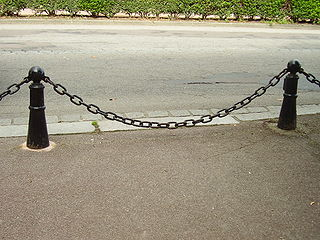
\includegraphics[scale=0.5]{figuras/catenaria.png}
		\caption{Kette Kettenkurve Catenary, Kamel15}
	\end{figure}
	
\end{frame}


\begin{frame}[label=conicas]{Por que o gráfico de uma função do $2^\circ$ é uma parábola?}
\begin{block}{Função do $2^\circ$ grau}
	\[f(x)=ax^2+bx+c, \ a\neq 0.\]
	\[y=ax^2+bx+c\]
\end{block}

\begin{exe}
Façao o completamento de quadrado e esboçe o gráfico de  
\[y=2x^2-12x+17.\]
\end{exe}

%Em particular, se $b=c=0$ e $a=1/4p$ temos que 
%\[y=\frac{1}{4p}x^2\Rightarrow x^2=4py.\]
\end{frame}


\subsection*{Cônicas Transladadas}
\begin{frame}[label=conicas]{Cônicas Transladadas}

\begin{center}
{\color{blue} Mudança de coordenadas }
\end{center}
\begin{equation*}
	\begin{cases}
		\textcolor{blue}{x'}=x-x_0\\
		\textcolor{blue}{y'}=y-y_0.
	\end{cases}
\end{equation*}

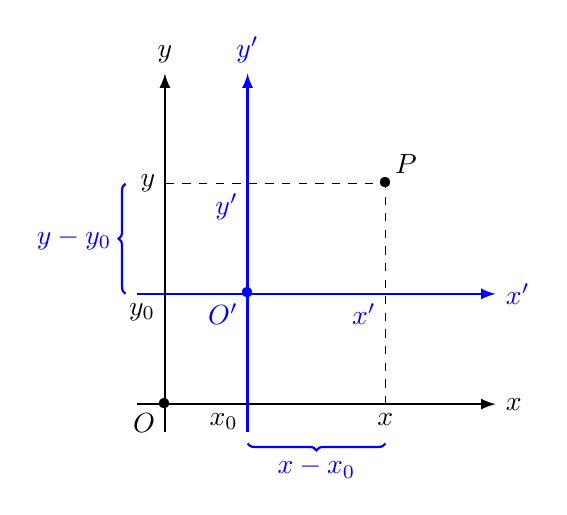
\begin{tikzpicture}[scale=0.7]

\usetikzlibrary{decorations.pathreplacing} 
\tikzset{>=latex}
%\draw[help lines, color=gray!30, dashed] (0,0) grid (6,6);

%sistema de eixos e ponto P
\draw[->,thick] (-.5,0)--(6,0) node[right]{$x$};
\draw[->,thick] (0,-.5)--(0,6) node[above]{$y$};
\node at (0,0) {\textbullet};
\node[below left] at (0,0) {$O$};
\node at (4,4) {\textbullet};
\node[above right] at (4,4) {$P$};
\draw[dashed] (4,0) -- (4,4) -- (0,4);
\node[below ] at (4,0) {$x$};
\node[left] at (0,4) {$y$};

%ponto de translação
\uncover<2->{
\node[blue] at (1.5,2) {\textbullet};
\node[below left,blue] at (1.5,2) {$O'$};
\node[below left] at (1.5,0) {$x_0$};
\node[below left] at (0,2) {$y_0$};
\draw[dashed] (1.5,0)--(1.5,2)--(0,2);
}


\uncover<3->{
\draw[->,thick,blue] (-.5,2)--(6,2) node[right]{$x'$};
\draw[->,thick,blue] (1.5,-.5)--(1.5,6) node[above]{$y'$};
}

\uncover<4->{
\node[below left,blue] at (4,2) {$x'$};
\node[below left,blue] at (1.5,4) {$y'$};

\draw[thick,decoration={brace,mirror,raise=0.5cm},decorate,blue] (1.5,0) --   (4,0)
node[pos=0.5,anchor=north,yshift=-0.55cm,blue] {$x-x_0$};
\draw[thick,decoration={brace,raise=0.5cm},decorate,blue] (0,2) --   (0,4)
node[pos=0.5,anchor=east,xshift=-0.55cm,blue] {$y-y_0$};}

\end{tikzpicture}


\end{frame}


\begin{frame}[label=conicas]

As equações de cônicas que não apresentam termos mistos da forma $xy$ 
podem  ser colocadas na forma reduzida através de uma translação de 
eixos.

\begin{exe}
Identifique e faça o esboço das cônicas a seguir:

\begin{enumerate}
\item $x^2+2y^2-6x+8y+9=0$.
\item $4x^2-16y^2-24x-24y+33=0$.
\end{enumerate}
\end{exe}

\end{frame}

\subsection*{Cônicas Rotacionadas}

\begin{frame}[label=conicas]{Cônicas Rotacionadas}
Os termos mistos da forma $xy$ de uma equação de cônica podem ser 
eliminados através de um processo de diagonalização, que equivale a uma 
rotação dos eixos.
\medskip

Uma expressão da forma
\[{\color{blue}a}x^2+{\color{blue}b}y^2+{\color{blue}c}xy\]
é chamada de \dt{forma quadrática} em $x$ e $y$ e pode ser representada 
usando matrizes da seguinte forma:
\[{\color{blue}a}x^2+{\color{blue}b}y^2+{\color{blue}c}xy=
\begin{bmatrix}
x & y
\end{bmatrix}
{\color{blue}\begin{bmatrix}
a & c/2\\ c/2 & b
\end{bmatrix}}
\begin{bmatrix}
x \\ y
\end{bmatrix}= X^t {\color{blue}A} X.
\]

\end{frame}


\begin{frame}[label=conicas]{Teorema dos Eixos Principais}
Como ${\color{blue}A}$ é uma matriz simétrica, pelo Teorema Espectral, 
existe uma matriz ortogonal que diagonaliza ${\color{blue}A}$, isto é, 
\[Q^t {\color{blue}A} Q={\color{red}D},\]
onde ${\color{red}D}$ é uma matriz diagonal formada por autovalores de 
${\color{blue}A}$.
Fazendo a \dt{mudança de variáveis} 
\[X=Q\bar{X}\ \text{ ou, equivalentemente, }\  \bar{X}=Q^tX,\]
temos
\begin{equation*}
X^t {\color{blue}A} X
=(Q\bar{X})^t {\color{blue}A}(Q\bar{X})
=\bar{X}^t(Q^t {\color{blue}A}Q) \bar{X}
=\bar{X}^t{\color{red}D}\bar{X}
\end{equation*}



\end{frame}

\begin{frame}[label=conicas]{Teorema dos Eixos Principais}
Assim, se ${\color{red}\lambda_1,\lambda_2}$ são os autovalores de ${\color{blue}A}$ e 
\[\bar{X}=
\begin{bmatrix}
\bar{x} \\ \bar{y},
\end{bmatrix}\]
então
\begin{align*}
{\color{blue}a}x^2+{\color{blue}b}y^2+{\color{blue}c}xy& =X^t {\color{blue}A} X\\
& =\bar{X}^t{\color{red}D}\bar{X}\\
& = {\color{red}\lambda_1}\bar{x}^2+{\color{red}\lambda_2}\bar{y}^2,
\end{align*}
uma forma quadrática sem termos mistos.

\end{frame}


\begin{frame}[label=conicas]
\begin{exe}
Identifique e faça um esboça das seguintes cônicas:
\begin{enumerate}
\item $5x^2+4xy+2y^2=6$.
\item $2x^2-4xy-y^2+8=0.$
\item $x^2+4\sqrt{2}xy-y^2+2\sqrt{6}x+2\sqrt{3}y=0$
\end{enumerate}
\end{exe}
\end{frame}


\begin{frame}[label=conicas]
\begin{casa}
Identifique e faça um esboço das seguintes cônicas

\begin{enumerate}
\item  $5x^2-4xy+8y^2-36=0$
\item $11 x^{2} + 24 x y + 4 x + 4 y^{2} + 3 y + \frac{15}{4} = 0$
\end{enumerate}
\end{casa}
\end{frame}

\begin{frame}[label=conicas]



\end{frame}




